\documentclass{article}
\usepackage{multirow}
\usepackage{float}
\usepackage{fancyvrb}
\usepackage{graphicx}

\title{\vspace{-2.0cm}BIOINF 704 Assignment 2}

\author{Badi James (bjam575)}

\begin{document}
	
	\maketitle
	
	\section{Accuracy of parameter estimation for logistic model of association:}
	
	\paragraph{}The logistic model is a way of modelling the association between two alleles (ie $A$ and $a$) at a locus and a binary phenotype (i.e trait that is either absent or present). It is described as follows: \\
	$p_g =$ probability that an individual of genotype $g$ has the trait. $g \in \{0,1,2\}$ assigned to genotypes $AA$, $Aa$ and $aa$ respectively. \\
	Log odds for $g$: \[= \log(\frac{p_g}{1 - p_g}) = \beta_0 + g \beta_1\]
	$\beta_0$ and $\beta_1$ are parameters that have to be estimated. The log likelihood of a given pair of values for these parameters can be calculated given a data set of genotype-phenotype pairs for each individual. First the above log odds equation is solved for each $p_g$. Second, the log likelihoods for each individual in the data having their phenotype given their genotype are calculated. Then these log likelihoods are summed together to get the log likelihood of the parameter values. With this a maximum likelihood (ML) approach can be taken when estimating values for $\beta_0$ and $\beta_1$.
	
	\paragraph{} However it is important to assess the accuracy of the parameter estimates. Estimating the variance of the parameters is a way of investigating this. This assignment demonstrates the non parametric bootstrap technique as a method of estimating variance.
	
	Using this data set $D$ of size $N = 31$:
	\begin{verbatim}
	phenotype:	1 1 1 1 1 1 1 1 1 1 1 1 1 1 1 1 1 1 1 0 0 0 0 0 0 0 0 0 0 0 0
	genotype:  0 0 0 0 0 0 0 0 0 0 1 1 1 2 2 2 2 2 2 0 0 0 0 0 0 1 1 1 1 1 2
	\end{verbatim}	
	$B = 100$ bootstap samples each of size $N$ were created by sampling with replacement from $D$. For each bootstrap sample, maximum likelihood estimates of $\beta_0$ and $\beta_1$ were found. This was done using the optim function in R, set to maximize instead of minimize, with starting values of $\beta_0 = 0.1$ and $\beta_1 = 0.2$. Otherwise default parameters for optim were used, meaning that the Nelder and Mead (1965) method was used to find the ML estimates. Then the variance of each $\beta$ was estimated using the formula:
	\[\hat{var}(\beta) = \frac{\sum^{B}_{b=1}(\beta_b - \bar{\beta})^2}{B - 1}\] 
	where $\beta_b$ is the estimate for the parameter for bootstrap sample $b$ and $\bar{\beta}$ is the mean estimate for the parameter across all bootstrap samples.
	
	\paragraph{}The results are:
	\[\hat{var}(\beta_0) = 0.1926\]
	\[\hat{var}(\beta_1) = 0.1715\]
	\[\bar{\beta_0} = 0.2260\]
	\[\bar{\beta_1} = 0.3533\]
	
	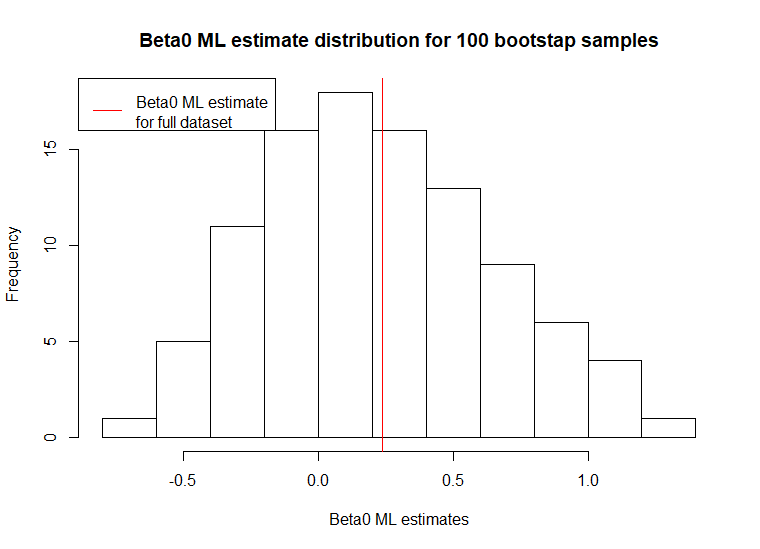
\includegraphics[scale=0.53]{Beta0}\\
	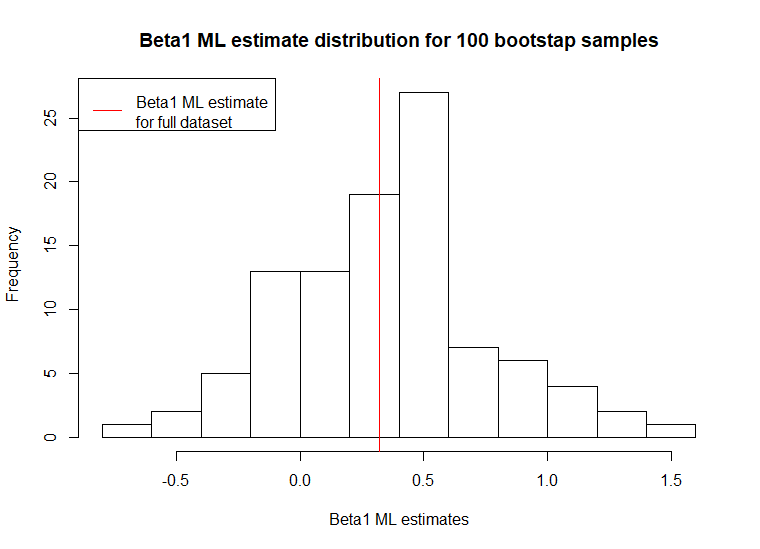
\includegraphics[scale=0.53]{Beta1}\\
	
	\paragraph{} As we can see the estimated variance for either parameter is not too extreme. The distributions of the estimates for each parameter are unimodal curves, with the curve for $\beta1$ being especially tall and narrow. From this we can judge that the parameter estimates are fairly accurate as the estimations for each sample tend to not deviate too far from the mean. Of note is the asymmetry of the distributions, which may be because of the asymmetry in the proportions of individuals with and without the phenotype and in the genotype frequencies. Of course, a larger data set would provide more accurate estimates. The non parametric bootstrap technique applied to a larger dataset would show less variance as the bootstrap samples would be less likely to skew the proportions of phenotypes for each genotype, and the distributions of the estimates would be taller and narrower.
	
	\section{SNPs in the FAMuSS study}
	
	\subsection{Testing SNP akt1 t10726c t12868 is in HWE}
	
	The function HWE.test from the R package genetics was used to test the null hypothesis that Hardy-Weinberg equilibrium holds for the alleles at this SNP across the population sampled. Its exact test for HWE gave a p value of $p = 1.091 \times10^{-6}$, suggesting with high statistical significance that the null hypothesis should be rejected and the alleles are out of equilibrium. However, when dividing the sample into sub populations defined by "Race", and testing each sub population individually (excluding "Am Indian" as there was only one individual belonging to that sub population) none of the p-values were below a significance threshold of 0.05 (Table 1). This is likely due to allele frequencies differing between sub populations. This would allow for HWE to hold for each sub population despite not holding for the full sample. This is an example of Simpson's paradox and why it is important to check for population stratification.
	
	\begin{table}[H]
		
		\centering
		\begin{tabular}{ll}
			Race       & p-value \\ \hline
			African Am & 0.2353  \\
			Asian      & 0.1201  \\
			Caucasian  & 0.8521  \\
			Hispanic   & 0.3241  \\
			Other      & 0.6612 
		\end{tabular}
		\caption{Tests for HWE at SNP akt1 t10726c t12868} \label{tab:title}
	\end{table}
	
	\subsection{Testing association between locus esr1 rs1042717 and BMI $> 25$}
	
	Using $\chi^2$ test across the whole sample:
	\[\chi^2 = 7.2638, df = 2, p = 0.02647\]
	This suggests rejecting the null hypothesis of no association as $p < 0.05$. However when testing each racial sub population individually (Table 2), the association is only significant for "Other". Fisher's exact test was used instead of $\chi^2$ for sub populations that had counts for a particular genotype with a particular phenotype that were $< 5$
	
	\begin{table}[H]
		\centering
		\begin{tabular}{lll}
			Race       & p-value & Test     \\ \hline
			African Am & 1*      & Exact    \\
			Asian      & 0.9109  & Exact    \\
			Caucasian  & 0.8958  & $\chi^2$ \\
			Hispanic   & 0.2196  & Exact    \\
			Other      & 0.0243  & Exact   
		\end{tabular}
		\caption{Testing association between locus esr1 rs1042717 and BMI $> 25$} \label{tab2:title}
	\end{table}
	
	\emph{*no AA genotypes were observed in the African Am sub population}
	
\end{document}